% Use standard two-column Latex article class with
% smaller margins and blank space for copyright notice

\documentclass[twocolumn,notitlepage,10pt,letter]{article}

% For pdflatex
\setlength{\pdfpagewidth}{8.5in}
\setlength{\pdfpageheight}{11in}

% Default margins are too big
% Magic below sets it to 1 inch all around
\setlength\oddsidemargin{+0.075in}
\setlength\evensidemargin{+0.075in}
\setlength\textwidth{6.5in}
\setlength\topmargin{-0.5in}
\setlength\textheight{8.5in}
\setlength\columnsep{0.33in}

\usepackage{float}



%\usepackage{dblfloatfix}
\usepackage{caption}
\usepackage{subcaption}
\usepackage{epsfig}
\usepackage{booktabs}
\usepackage{tabularx}
\usepackage{url}
%\usepackage{adjustbox}
\begin{document}

\title{\Large \bf Weighted Dice: An Evaluation of System Security in the Face of Limited Entropy}

\author{
  {\rm Daniel A Cashman}\\
  University of California, San Diego
} % end author
\date{} % no date on first page
\maketitle


\subsection*{Abstract}
\textit{A lack of entropy gathering devices on some headless and embedded Linux systems has led to an early window during booting wherin values produced by the Linux PRNG are more easily predicted.  We identify and describe four sources of randomness in the kernel, including the Linux PRNG. We also identify an unaccounted source of entropy due to variation in request ordering of the Linux PRNG non-blocking pool.  Finally, we perform an analysis of the security level of four kernel-based security mechanisms dependent on random values: TCP sequence numbers, UDP source ports, stack canaries and ASLR.  We conclude that good random values should be a system responsibility and that the current design of sources providing random values should be consolidated and changed to reflect a more practical threat model.}


\section{Introduction}
Randomness is a well-known feature of modern cryptosystems, which depend on random numbers for security.  Unfortunately, generating truly random numbers is a hard problem due to the determinstic nature of computers.  Current systems rely on Pseudo-random number generators (PRNGs) to generate numbers that appear to be random to outside applications, but despite a great deal of research, their implementation is also difficult and they have often failed \cite{linuxPRNG, yilek, netscape, poker, java_sessid, bellare_dss, chor_bits, windows}. A recent study by Heninger et al. identified one such failure in the use of the Linux PRNG for certain headless and embedded systems, in the form of a boot-time entropy hole, wherein a lack of sufficient random seeding early on in the boot process led to the adoption on those systems of weak, repeated crytographic keys \cite{pnqs}.  In this paper, we investigate the generation of random numbers in the Linux kernel and explore other, non-cryptographic, security implications of such a boot-time entropy hole.  

PRNGs base their future output, which would be predictable otherwise, on random seeds.  Hard-to-predict events such as the timings of user input activies, disk accesses, and interrupts generate the values of these seeds\cite{disk_timing}. In the Linux PRNG this seeding is accounted for by the notion of entropy, which represents the perceived true level of randomness of the seed.  Given current cryptographic methods and computing power, approximately 200 bits of entropy is currently deemed enough to generate an output which is effectively random to observers \cite{tcp_RFC}.  

The paper by Heninger et al. revealed that in certain headless and embedded systems, the estimate of entropy in the Linux PRNG did not reach 128 bits until more than 30 seconds after boot, and furthermore that no entropy seeding was given to the non-blocking pool, the one from which the kernel gets its random values, until the gathered entropy estimate reached 192 bits, approximately 66 seconds after boot.  This window of low entropy at boot-time is large enough to affect practically every process which relies on random values during boot-up.  

This paper describes the general operation of the Linux PRNG and reveals the existence of multiple, previously unknown to us, entropy pools within the kernel.  It also presents an analysis of multiple security mechanisms in the presence of a boot-time entropy hole.  Specifically, we were able to take advantage of poor randomness in the networking code to spoof TCP connections, IP identifier fields and UDP source ports.  We also attempted to circumvent two low-level security mechanisms: stack canaries and address space layout randomization but were thwarted due to the use of one of the aforementioned newly discovered entropy pools instead of the low-entropy Linux PRNG.  
In the next section, we describe the basic operation of the Linux PRNG.  Section 2 also describes the other entropy pools we encountered during our analysis.  Section 3 details our efforts to reproduce the boot-time entropy hole discovered by Heninger et al.  Sections 4 - 7 discuss our exploitation attempts: TCP spoofing in section 4, stack canary circumvention in section 5, ASLR prediction in section 6 and DNS poisoning in section 7. Section 8 is our conclusion, and section 9 discusses related and suggested future work.








  


\section{An Overview of Sources of Randomness in the Linux Kernel}
A good deal of previous work has been written about \textit{the} Linux PRNG, which refers to the code which generates user-acccessible random bits via /dev/random and /dev/urandom\cite{linuxPRNG, revisited, viega, pnqs, kmowery, random4}.  This wording is misleading, however, as it ignores other sources of random values inside of the Linux Kernel, including even the random32.c Tausworthe PRNG, closely related to \cite{random3}\cite{tausworthe}.   Though our work is also based primarily on the PRNG associated with /dev/random and /dev/urandom, still referred to henceforth as the Linux PRNG, we also describe here three other entropy pools we encountered during our investigation into the effects of low boot-time entropy on system security.

\subsection{The Linux PRNG}
Due to our desire to further explore the implications of the findings from Heninger et al., our work was done on the same 2.6.32.57 Linux kernel, which was the same version, 2.6.32, used in their work.  The basic structure of the PRNG has remained fairly constant, however, with the main components essentially unchanged in the last few years, and a more detailed explanation from a slightly older version may be found in Gutterman and Pinkas\cite{linuxPRNG}.  The differences between 2.6.32, our test version, and the latest stable release at the time of writing, are primarily limited to additional methods of adding entropy input, which were added in response to the discovery by Heninger et al. of the boot-time entropy hole herein discussed. Thus, the following discussion should be applicable across many different Linux versions. 

The Linux PRNG can be viewed as being comprised of three principle components: a component to maintain and modify the state of the PRNG, a component to add entropy collected by events in the outside system,  and a component to generate output when requested.  The state of the PRNG is maintained as three distinc pools, or stores of bits.  Of the three pools, one is a 512 byte \textit{input} pool, and the other two are 128 byte \textit{output} pools.  The two output pools differ in response to insufficient estimated entropy: the non-blocking pool reads data from the pool in all situations, whereas the blocking pool will block until enough is available.  A read of the system timekeeper provides a number of seconds and nanoseconds with which to initialize the pools.  Entropy events first add bits to the input pool, which may then be passed to the output pools on request, so that they may then serve bits to a requesting application.  The latest kernel version adds these values to the non-blocking pool instead to avoid the low-entropy hole \cite{kmowery}. Each pool has an associated estimate of the amount of entropy contained therein, which is always initialized to zero, and then incremented or decremented as it gathers system randomness and provides output to consumers, respectively.  Each pool also has an associated primitive polynomial, which is used by the mix\_pool\_bytes() function to stir the pool contents whenever its state is changed.  

The portion responsible for adding entropy to the PRNG is essentially the source of randomness for the system.  Computers operate on a fixed set of rules and generate output determinstically from given inputs. The entropy adding component utilizes the timings and values of hard-to-predict, non-determinstic events to introduce this randomness.  In the 2.6.32 kernel, entropy may be collected from disk, input and interrupt timings, though interrupt timings were disabled by default.  As of the latest stable release, interrupt timings had been reenabled and augmented with a fast\_mix() function, and a new function, add\_device\_randomness(), had been added to provide additional unique values to directly combat, again, the boot-time entropy hole at the foundation of this paper. Each entropy event is added to the pools by recording the jiffies count, cycle count and the value associated with the the entropy event itself, such as the key-value on a keyboard press, in a sample and then mixing that 12-16 byte, depending on architecture, value into the input pool by mix\_pool\_bytes().  The amount of estimated bits of entropy added to the pool is dependent on the type of input, and the entropy estimate for the input pool is credited the corresponding amount of bits.  User applications may also mix in data by writing to /dev/urandom or /dev/random, which mix the provided data into the appropriate pool, but do not add to the entropy estimate.

The final component of the Linux PRNG deals with extracting output from the entropy pools, which may be done via three interfaces:  /dev/urandom, /dev/random, and get\_random\_bytes().  /dev/urandom and /dev/random are user-accessible device drivers which read their output from the non-blocking and blocking pools, respectively.  get\_random\_bytes() is the interface used by requests for random data from within the kernel itself, and it too reads from the non-blocking pool. When output is requested of either the blocking or non-blocking pool, a check is first made to see if the entropy count in the current pool is great enough to satisfy the request; if not, a request is made for bytes from the input pool.  The input pool will transfer no more bytes than it has credited entropy, minus a minimum value to keep, to one of the output pools. After the transfer from the input pool, if it was needed, the new entropy count of the output pool is derived and then that number of bytes is extracted.  In the case of the blocking pool, no more than the entropy estimate can be extracted, but the entire requested number may be extracted from the non-blocking pool.  The entropy estimate of the output pool is then decreased accordingly.  The blocking pool repeats this process until it has been able to generate enough bytes as requested by the user. The actual method for extracting data from any of the three pools for consumers involves repeatedly hashing different portions with SHA1 and a 20-byte output buffer, which is mixed back into the pool and folded onto itself to produce a 10-byte output. Bytes must be repeatedly extracted in 10-byte chunks until the request is fulfilled.

\subsection{Tausworthe PRNG}
Another, completely separate PRNG is found in lib/random32.c.  Like the non-blocking pool in the Linux PRNG, it is declared to be unsafe for cryptographic use:
\\
\texttt{
/**                                                                             
       A 32 bit pseudo-random number is generated using a fast                 
       algorithm suitable for simulation. This algorithm is NOT                
       considered safe for cryptographic use.                                  
 */
}  
\\
It too may be divided into the three components mentioned for the Linux PRNG.  The state of this PRNG is maintained by a per-CPU variable called net\_rand\_state, which is just a structure of three unsigned integers.  The system jiffies count is the basis of the first initialization of the PRNG, but as noted in the code, this is extremely weak and likely to be the same across boots.  To combat this, the state may be reseeded after the Linux PRNG is initialized by a call to get\_random\_bytes().   The system entropy events which provide values to the Linux PRNG, described above, do not interact with the Tausworthe PRNG, but entropy may be selectively added by calls to srandom(). srandom() simply XORs the provided unsigned integer with the first one of the PRNG state.  Output from the PRNG is generated by a Tausworthe transformation of each of the three state unsigned integers, which are then XOR'd together.

\subsection{get\_random\_int}
We found a third PRNG, get\_random\_int(), which we encountered during our investigation in the same file as the Linux PRNG. Like the Tauseworthe PRNG, this also relied upon a per-CPU variable and was declared to be unfit for cryptographic use, but more troublingly indicated a misunderstanding of the nature of entropy regarding PRNGs. 
\\
\texttt{
/*                                                                              
  Get a random word for internal kernel use only. Similar to urandom but       
  with the goal of minimal entropy pool depletion. As a result, the random     
  value is not cryptographically secure but for several uses the cost of       
  depleting entropy is too high                                                
 */
}
\\

   The state of this PRNG is simple a pool of 16 bytes, large enough for use with the MD5 hash.  Its state is initialy zeroed memory, but it collects entropy at each request for output by combining the system jiffies count, the process ID and the current cycle count into the first 4 bytes of the pool and then setting the pool to an MD5 hash of the result.  The output generated is the first four bytes of the pool after the hashing.

\subsection{net\_secret}
The final source of randomness we encountered, net\_secret, could not properly be described as a PRNG, but was, nevertheless, used to generate random values.  net\_secret is a 64-byte pool initialized during the boot process by a call to get\_random\_bytes().  Unlike the other sources of randomness, though, its value is never updated, despite a waring in \cite{tcp_RFC} that this should be done occasionally.  Its state is used in combination with an MD5 hash, however, to generate random values for portions of the networking code in combination with the current time and other connection-specific inputs.  


\begin{figure*}[htb]
        \center{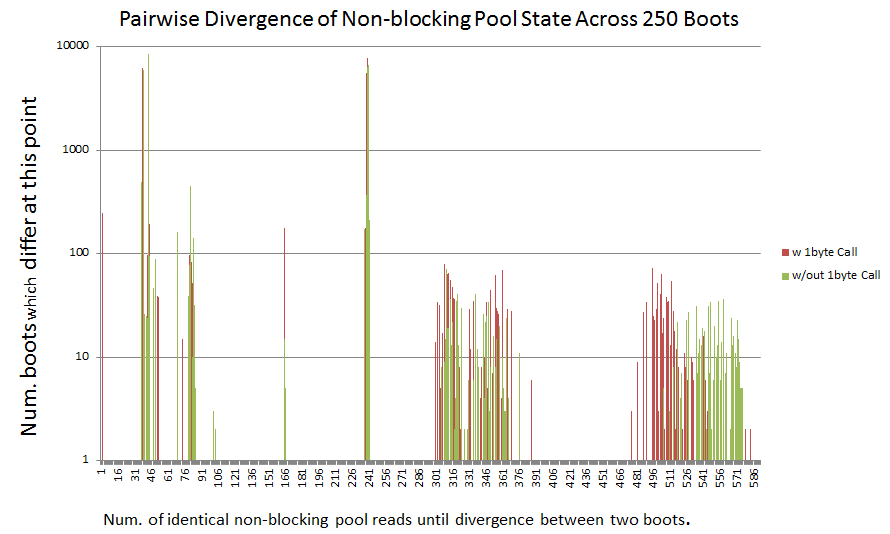
\includegraphics[width=\textwidth]
        {implicit_entropy_graph.png}}
        \caption{\label{fig: label} 250 boots on our Ubuntu machine had the state of their non-blocking pools output at every read and change and subsequently compared to all other boots.  This figure indicates where the non-blocking pool states diverged between every pair of boots.}
\end{figure*}

\section{Reproduction of the Boot-Time Entropy Hole}
We first tried, with partial success, to see if we could accurately replicate the low-entropy output found in Heninger et al, and in the process of doing so discovered a source of implicit entropy in the non-blocking pool.  To do this, we first attempted to replicate their environment.  We used Linux version 2.6.32.57 and compiled it on both a VMware virtual machine running Ubuntu desktop 12.04, with 1GB of RAM and 1 processor, and an hp pavillion running Ubuntu Server 10.04, but due to mechanical failure, replaced our pavillion with a Lenovo Thinkpad R61 running Slackware 13.0 instead. We modified the Linux PRNG so that it was zeroed at initialization to simulate a cold boot, initialized the timesource in the kernel to zero to simulate the lack of a working clock, and limited the machine to using only one processor to simulate a simple headless embedded device, all in accordance with the findings of Heninger et al.  We were unable to reproduce their exact results, but discovered a source of what we define as \textit{implicit entropy}, which is simply a source of entropy unaccounted by the PRNG. 

Once set-up, we ran 1000 boots under these conditions and recorded 4 and 128 bytes of output from /dev/urandom.  Unfortunately, we did not find any repeated readings, in contrast to the only 27 values found by Heninger et al. To account for this disparity, we recorded a summary of the state of the non-blocking pool in the Linux PRNG each time its state was modified.  The difference between the state of the non-blocking pool compared to all other boots is shown in figure 1, with the state between boots diverging at different clusters of reads.  We found that the estimated entropy of the non-blocking pool was zero for the entire duration of our boot until reading from /dev/urandom, and that the estimated entropy for the input pool reached, on average 138 bits on our Ubuntu system and 155 on our, much slower, Slackware one.  At the point where the state of non-blocking pool diverged between boots, though, the input pool also had zero entropy, meaning that no gathered entropy was being transferred to the non-blocking pool.  The only source of change for the pool's contents was the hashing and mixing triggered on each output request. 

Therefore, the difference in values between boots could only by explained by the order in which output requests were made, which acts as a source of implicit entropy gathering, similar to the race conditions discussed by Heninger et al \cite{pnqs}.  Due to the folding back into the pool of hashed output, a change between boots in the number of previous requests for any new request will lead to it obtaining a different output value.  The value read may even be different if the number of previous requests is constant, however, if the ordering of the previous requests is different.  This is because the pool stirring for each read is a function of the bytes requested, and so the pool state after a read of \textit{x} bytes followed by a read of \textit{y} bytes will not be the same as the pool state after a read of \textit{y} followed by \textit{x}, provided \textit{x} and \textit{y} are different values. If the reads are for the same number of bytes, though, then the state of the pool will be the same after any ordering. 

We found that the vast majority of requests for data from the non-blocking pool, 494 out of 552 reads on our Slackware system and 826 out of 854 on our Ubuntu system, were 16-byte get\_random\_bytes() calls, meaning that the ordering of the remaining calls was responsible for the variation we encountered.   What's more, the diversity of non-16-byte requests was fairly low; 31 of the 58 calls responsible on our slackware system, 7 of 28 on Ubuntu, for the implicit entropy we observed came from the same origin.  Disabling just that source resulted in the non-blocking pool state diverging between boots later than with it included.  This is shown in figure 1, which shows the non-blocking pool state on our Ubuntu machine (our Slackware machine was slow enough that almost all divergence happened after only the 39th read).  For perspective, our read of /dev/urandom occured always occured after the 543rd read and before the 547th read for our Slackware system, and after the 878th and before the 921st on Ubuntu.  Likewise, the seeding of the Tausworthe and net\_secret sources of randomness occured at approximately the 6th and 7th requests, respectively.  These requests were before any divergence across boots, a fact of which we made use in sections 4 and 7.  Thus, we were able to replicate deterministic results under the given assumptions, but to a lesser-degree than found by Heninger et al. A system configured without a large subset of these sources of implicit entropy generating non-16-byte requests, however, would be without the implicit entropy found therein, and should lead to a smaller range of possible output values while entropy from normal sources is being gathered.





\section{TCP Sequence Number Spoofing}
Nearly any modern system for which security is a concern is connected to a network, but many of the protocols used for networking were not designed with security in mind.  The TCP/IP protocol suite, at the heart of most communication on the Internet, is an example of exactly this situation\cite{tcp_problems_back, tcp_attacks_methods}.  TCP, the transimission control protocol, is a packet-based transport level protocol, built on top of the IP layer, which maintains a connection between endpoints.  The establishment of a TCP connection allows for more advanced features, such as dealing with packet loss, duplicates and errors, than are available with connectionless protocols such as UDP \cite{illustrated}. Knowledge of a TCP packet's sequence number is all that is required to \textit{spoof} a connection, so randomization is used as a security mechanism against this\cite{tcp_RFC}. We found that in the face of low-entropy, though, this mechanism fails. 

A TCP connection is defined by the IP address and port number of each end-point, allowing each connection to be represented by a unique 4-tuple of those values.  Connections are opened via a process called the \textit{three-way handshake}.  To begin such a handshake, a SYN packet request is sent with an initial sequence number from a client-side IP address and port to a server listenning on the destination port at the indicated IP address. When a SYN packet is received by a listenning server, a response is sent consisting of its own sequence number, and the originally received client sequence number incremented by one, called an ACK.  Finally, after receiving the server's response, the client sends another packet with its original sequence number, and the server's original sequence number, both incremented by one.  Upon receipt of this third packet, data packets are free to be transferred between client and server with the sequence numbers incremented according to the bytes sent and acknowledgements incremented according to those received.

Each end of the connection only sees what is contained in the packets it receives.  The 4-tuple defining the connection and the appropriate sequence and ACK numbers are all that are required to be accepted at either end, potentially allowing an adversary to send forged packets.  Randomization of the initial sequence numbers for client and server, in addition to an assumption that there is no man-in-the-middle listenning in, is designed to make spoofing connections in this manner difficult.  

In the face of a boot-time entropy hole, the randomness of the initial sequence numbers is very weak. The transport layer is created by the kernel, and as a result, TCP sequence numbers are generated by it as well.  Investigation revealed that a connection's TCP sequence number is a function of the state of the net\_secret source of randomness described in Section 2, the time of its creation, and the 4-tuple defining the connection to which the TCP packet belongs. This was also the case for IP identifiers, but without even a timing component.  Specifically, the 4-tuple is combined with the net\_secret as input to an MD5 hash, whose output is combined with the time information.  As explained in the previous section, the initialization of net\_secret in a low-entropy boot occurs early enough such that its value is the same for each boot. Since the state of the net\_secret is never changed, an adversary with access to the same type of device as the target system only needs to determine the time of packet creation to replicate sequence number generation.

Using the information available to an adversary, we were able to craft an attack which can spoof an arbitrary TCP connection. We first sent a legitimate connection request to the target server to establish a connection.  Given that we already knew the net\_secret state, the 4-tuple, and the MD5 algorithm, we were able to generate a sequence number without any time component.  By subtracting this from the actual sequence number, we were able to deduce the current time component being added.  We then measured the increase in this time component by sending a series of other legitimate data packets to deduce the amount of time being added by the round-trip delay.  Finally, we created a sequence number using the net\_secret and the 4-tuple of the connection we wished to spoof, and added to it the timing component and expected round-trip delay to successfully spoof our desired connection.  This spoofing was successful only for systems for which we could deduce an accurate component for the round-trip delay; systems which used the tsc timesource, for instance, had a timing component that was fine-grained enough to notice differences between the round-trip delay of each packet.  The devices which exhibited the boot-time entropy hole are unlikely to have such high-precision timesources, however, and thus should be susceptible to this attack.  

In addition, we were able to modify our spoofing attack to actually create a probe to uncover systems with the boot-time entropy hole.  We followed the same procedure as in the spoofing attack, but instead of choosing a connection to spoof, we simply made a second legitimate connection with a different 4-tuple so that we could observe the actual sequence number.  Since we already determined the expected sequence number for the second connection in the case of a known net\_secret due to low entropy, if the observed sequence number matched our expected sequence number, we could identify the system as one with low-entropy, and possibly open to other attacks as a consequence.   


\section{Stack Canary Randomization}
Another area in which randomization is used to enhance security, is in the use of stack canaries to defend against perhaps the most iconic of software vulnerabilities: buffer overflows \cite{stackguard, stackguardUse}.  Though widely known since the Morris Worm in 1988, buffer overflow vulnerabilities persist to this day and may present attackers with an opportunity to take complete control of a vulnerable system \cite{buff_overflow_today}. Buffer overflows are of a class of vulnerabilities which rely on the layout of  data in memory, with attacks exploiting the storing of return addresses in stack frames alongside local data \cite{aleph, lowLevSec}. 

Specifically, during program execution, each new function invocation results in the program counter value being changed to the memory location of that function, which requires that the location of the instruction which called the new function be saved to enable execution to return there after the new function finishes. In assembly, this is represented by the function prologue and epilogue, which manage stack frames and change the address stored in the program counter.  Automatic variables, including local arrays, are also stored on the stack and may have their values changed during execution.  A lack of bounds checking when writing to these automatic variables may lead to other addresses being overwritten, as is the case when strcpy() copies characters from a string into an array for which it does not have enough room.  In this case, a buffer overflow has occured, and if enough data was overwritten to also overwrite the stored return address of a calling function, then when the function epilogue restores the program counter using it, the program execution will continue by fetching instructions at the address specificed by its new value.  If an attacker is able to place a memory address of his/her choosing in place of the return address, then he/she may execute code anywhere in the process's address space; this often results in the launch of a root shell specificed by code the attacker placed, or pieced together, elsewhere in memory.

Stack canaries, such as that proposed by Cowan et al in the case of StackGuard, attempt to prevent such overflows by introducing a \textit{canary} in between the automatic variables of a function and the data saved by the function prologue \cite{stackguard}.  The canary consists of a value which is checked in the function epilogue prior to loading the the stored return address into program counter.  If the canary does not still have its original value, then execution is not allowed to continue and the program crashes, rather than directing control do a new, potentially dangerous, region of memory.  As a result, the canary value is randomized to make it difficult for an attacker to replicate it as part of a buffer overflow exploit.  In order to provide an effective defense, the canary value must be different each time the program is run.  On Linux systems, the responsibility for generating the random canary value lies in the kernel, and thus could be affected by poor entropy at boot time.

Our investigation into the security of stack canaries in the presence of low-entropy at boot time began with the observation that one of the very first function calls in start\_kernel() at the very beginning of the linux boot process was a call to boot\_init\_stack\_canary(), which established the stack canary of process 0, running start\_kernel().  This call is made well before the linux PRNG is even initialized, and so would be expected to be deterministic if not relying on other sources of entropy.  Due to reliance on the architecture-specific tsc counter, which would not be present in systems with the boot-time entropy hole in which we're interested, in a special implementation of boot\_init\_stack\_canary() for the x86 machines, we decided to perform our investigation on the ARM architecture instead, which initializes via a call to get\_random\_bytes() from the Linux PRNG.  We used an available Raspberry-Pi B model machine for this purpose.  The special ARM architecture from Broadcom on the machine required us to change to the Raspbian Linux Kernel, of which we chose the most recent 3.6.y.  Changing kernel versions was necessary, we discovered, because the boot\_init\_stack\_canary() code was not implemented for non-x86 architectures in our 2.6.32.57 kernel, anyway.

We recorded this first stack canary from the call of boot\_init\_stack\_canary() and discovered that the initialized value was the same across all boots.  To determine if this early-initialized canary value persisted and ascertain a potential exploit, we wrote a kernel module with a simple buffer overflow vulnerability using get\_usr() without proper bounds-checking. Examination of the stack when calling the function with the vulnerable buffer allowed us to locate the canary and the protected return address. With this information, we successfully wrote an exploit that directed control flow to a different kernel function of our choosing, but unfortunately, we verified that the canary differed from the early-initialized one.  As a result, we were only able to craft a successful exploit when also examing the memory layout directly.  A search through the kernel revealed that a new stack canary value is generated by a call to get\_random\_int(), described in Section 2, upon the forking of every new process when duplicating the process structures.  Thus, since the canary value initialization is completely independent of the Linux PRNG, despite the reliance of the first canary in boot\_init\_stack\_canary() on it, we were unable to defeat the stack security mechanism on a system with low boot-time entropy.  


\section{Address Space Layout Randomization}
Stack canaries, as a low-level security defense, are only capable of thwarting attacks which rely on clobbering return addresses.  Other defenses, such as non-executible stacks and control flow integrity have been established, but are themselves vulnerable to various combinations of other attack vectors, such as function pointers, data contamination, return-to-libc, heap overflows, and more \cite{lowLevSec, freeVuln, format, intOverflow, cfi}.  A completely different defense, Address Space Layout Randomization,  recognizes that these memory-based vulnerabilities are extremely delicate, and may be rendered completely ineffective if the address calculations therein are off \cite{PaX}.  As the name implies, it changes the memory layout such that the program's symbols are mapped to different addresses at each invocation, which is enough to foil the previously mentioned address calculations.  ASLR is now a widely accepted defense mechanism that is still being deployed to new platforms, but suffers when not supplied with sufficient randomness \cite{android_ASLR, ASLP}.  We found that our Linux boot-time entropy hole had no effect upon ASLR, but instead that a different entropy pool was being used to generate its values.

The address space of a process is established when its binary object is loaded from disk by the operating system, and is shared by any process it forks which does not subsequently execute a different program \cite{linkers_loaders}.  We sought to determine if low-entropy in the Linux PRNG could compromise the ASLR of processes loaded early in the boot process.  This required an examination of the ELF loader in the Linux Kernel, which revealed that address spaces for ELF objects are randomized into four principle regions: the text segment, heap, dynamically loaded libraries, and the stack.  

Unfortunately, due to relative address calculations, page table boundaries, and other considerations, ASLR is limited to course-grained randomization, rather than being able to assign each symbol a completely random address\cite{ASLR}.  Thus, while the exact address of a vulnerable buffer may change between program invocations, its location to the stack frame, for example, would remain the same.  In practice, this has meant that ASLR has been vulnerable to brute force attacks due to its inability to use a full 32-bits of entropy for its randomization, but it still presents an effective barrier in situations where this is difficult. 

For our analysis of ASLR in the presence of low-entropy, we installed the Apache web server to allow us to insert and exploit a simple buffer overflow vulnerability similar to the one used in \cite{ASLR}.  The use of Apache was important because it forks child processes to deal with incoming requests, which results in them having the same memory layout as the parent process, a layout established during boot-time.  We then identified the locations in the code of the ELF loader where the text segment, heap and stack base addresses were assigned random values.  The linker-loader and dynamically loaded libraries relied on the kernel do\_mmap() function, which used a random base address determined for the process when do\_execve() is called.  We were surprised to find that none of the ASLR random calls made use of the Linux PRNG, but rather relied on the get\_random\_int randomness source, described in Section 2.  Despite not making use of our boot-time entropy hole, we had hoped that the perceived lack of strength of this randomness source would enable us to effectively circumvent ASLR.

We compared the random values read in the kernel with the output of the memory layout as read by /proc/PID/maps to confirm their role in ASLR.  Once established, we then compared the address space of our Apache process across boots, and repeated for 1000 boots for the init process, which receives its values much earlier.  An interesting side-effect of this was the discovery that the dynamically linked libraries were always in the same positions relative to each other, meaning that do\_mmap() uses only the initial randomization to assign new addresses.  Otherwise, the Apache ASLR generated different memory layouts every time.  This was a side-effect of a gathering of implicit entropy similar to that observed for the non-blocking pool in Section 3.  By the time our Apache process requested the random values for its address space, the get\_random\_int PRNG had produced output over 3000 times, with each read adding its hashed output back into the pool as described in Section 2.  In contrast, the address space of the init process on our modified Slackware system had effectively the same unique address space on every boot, a side effect of getting its values from the first few reads of the get\_random\_int PRNG.  Interestingly, we did not observe any overlap on our Ubuntu machine.  Thus, our attempt to use low boot-time entropy to defeat ASLR failed for our Apache target due to an unexpected, but heavily used, entropy pool.  ASLR protection of earlier processes, such as the init process, however, contains practically no randomness, and may be an issue as early sophisticated processes begin to replace the init process. 


\section{DNS Poisoning}
Another critical part of the Internet which relies on randomization for security is the Domain Name Service (DNS).  DNS is responsible for translating fully qualified domain names, represented as a series of characters separated by periods, such as www.example.com, into numeric IP addresses, such as 1.2.3.4, which are in the form actually used by computers \cite{illustrated}.  Since directly manipulating IP addresses is difficult for humans, DNS is an important component at the heart of the modern use of the Internet, and has correspondingly received attention from malicious users.  A large portion of malicious online activity, such as phishing, click-jacking and cross-site request forgery, is centered around getting users to visit domains which are under a hacker's control\cite{phishing, csrf, clickjack}.  DNS presents another opportunity to do this by associating a popular domain name, like that of a major financial institution, with an attacker-controlled IP address, in a process called DNS poisoning, instead of an authentic one to which it would normally be assigned \cite{DNSPoison}.  Current defenses against DNS poisoning are based on randomization, which is weakened on systems with low boot-time entropy.

DNS is based on a hierarchical system in which a name server is considered an authority on address translations for its own domain(s) and those below it.  Such a name server may know the addresses of other name servers, which in turn know information regarding their sub-domains, and so on.  A query for the address of www.example.com would result in a query of the root server '.' which would give the address of the name server responsible for translations of the .com namespace, which would in turn refer to the nameserver responsible for example.com, and finally to one for www.example.com, which would provide the final IP address translation.  Thus, a look-up of a domain name could take multiple queries.  To alleviate this overhead, translations for the different steps are often cached, preventing the need for repeated look-ups for the same domains.   

DNS poisoning is the process of populating just such a DNS cache with an unauthentic translation of an attacker's choosing.  In its simplest form, this simply required an attacker-controlled DNS resolver to issue a query to a recursive name-server for the domain name to be poisoned and then answer the recursive name-server's subsequent request to name-servers further up the hierarchy before they responded.  To answer the query successfully, the attacker must have matched the DNS query ID, a 16-bit field in the DNS header.  Randomization of this number made DNS poisoning more difficult by reducing the probability of a successful attack to a function of the number of queries that could be made before an authentic response was received and cached, precluding more attacks on that domain name for the cache duration.  The Kaminsky attack, however, got around this by instead sending queries for random domain names with the goal of successfully forging a response for a name-server update\cite{kaminsky}.  The attack could be performed on many domains in parallel and, when properly crafted, would give the attacker complete control of the name-server, and thus enable them to poison the response for an arbitrary domain.  To mitigate this, the source ports of the UDP packets from which the DNS queries were made were then also randomized, to require an extra 16 bits, in addition to the 16 from the DNS ID field, that an attacker would have to know to successfully forge a response.

We desired to determine if these two values, the UDP source port and the DNS query ID, could be more easily determined on systems with the entropy deficiency described earlier.  For the DNS query ID we examined the source code of the resolver provided in version 2.11.1. of glibc, the C standard library on our test machine, with the hope that its randomness was derived from a call to /dev/urandom.  Contrary to our expectations, however, the randomness of the DNS query id field was provided by a combination of resolver's process id and, in the absence of a high precision timer for use with glibc, a get\_time\_of\_day() system call.  Specifically, the seconds returned were left-shifted 8 bits and then XOR'd with the microseconds returned.  Thus, at least for the DNS query ID,the linux PRNG was uninvolved.

The assignment of the UDP source port for requests is set by the Linux Kernel, but a desired source port may be indicated by the user process.  We first measured the value passed by the glibc resolver to confirm that randomization was not being done in user-space, but was rather left to the kernel.  With this confirmed, we traced the randomness associated with the assignment of the UDP source port to a call to net\_random().  Surprisingly, net\_random() is based on a call to a completely separate kernel PRNG located in lib/random32.c, which is based on the Tausworthe linear feedback shift register, described in Section 2.  We found that this PRNG was initially seeded with a self-described weak seed, based on the jiffies count of the system, but was reseeded later after initialization of the normal linux PRNG, with a call to get\_random\_bytes().  This later reseeding was done at only the 6th read from the non-blocking pool, right before the initialization of the net\_secret, as previously discussed in Section 3, and was not observed again on our Slackware system.  Our Ubuntu system, however, reseeded the pool four times during the initial boot.  As a result, the observed initial state of the PRNG in random32.c was identical across all boots in our low-entropy tests for our Slackware system.  

Furthermore, the state of the PRNG only changed when entropy is added via an srandom32() or if a call to random32() stirs it.  In our tests, entropy was only added to the PRNG by four different calls made by ifconfig during initialization, and the entropy seed values were the same for each call across boots.  As a result, we observed the same sequence of UDP source port assignments on every boot.  These findings indicate that an attacker with a properly configured system could be able to determine UDP source port numbers by simply keeping track of the number of UDP packets sent since the low-entropy target system last booted, or observing a series of UDP source port numbers and mapping them to an appropriate place in a pre-configured sequence.  Thus, systems with low boot-time entropy lose the additional protection of randomized UDP source port in DNS transactions and would again be vulnerable to DNS poisoning.


  







\section{Conclusion}
In this paper, we examine the effect of low boot-time entropy in the Linux PRNG on a selection of randomness-dependent security mechanisms.  Previous work had already shown a significant impact of poor boot-time entropy on system security by measuring an extremely poor distribution of values for cryptographic purposes, an obvious and critical area in need of good randomness.  We show that poor randomness is a problem that extends beyond cyrptography and can lead to security vulnerabilities in other areas.  Specifically, we are able to predict sequence numbers to spoof TCP connections and scan for systems with low boot-time entropy.  We are also able to eliminate the extra layer of security proved by random UDP source port numbers in DNS queries, and to observe a greatly decreased reduced number of possibilities for address space layout randomization for processes which are spawned at the very beginning of the boot process.

We also provide an overview of four different sources of randomness for security critical consumers, only one of which receives entropy inputs from standard hard-to-predict events.  Our interactions with these sources of randomness show that a lack of diversity in requests from PRNGs, a failure to incorporate output back into PRNG state, and a paucity of entropy seeding may all result in vulnerabilities in security mechanisms.  We observe that, in pools which incorporate their output into their state, a heretofore unaccounted source of implicit entropy based on request ordering adds a significant amount of variability later in the boot process, even when no other sources of entropy are present.  

Our observations lead us to believe that the provision of randomness from the kernel should be redesigned according to more modular software engineering and a new threat model.  Our first recommendation is that the four sources of randomness in the Linux kernel be consolidated into only one source which acts as a provider for the entire operating system and user applications.  The division of responsibility between different sources necessarily prevents the maximum use of entropy for all applications.  The ordering of the 3000-plus get\_random\_int() calls alone would introduce a large amount of implicit entropy to the Linux PRNG, which could be increased by incorporating cycle counts every time the pool is mixed, as is done with the get\_random\_int() entropoy pool.  The maintenance of only one source would also developers to focus on making certain that the one source is properly maintained.  This would help avoid simple errors such as the elimination of state reseeding for net\_secret between the Linux 2.4 and 2.6 kernels. 

In addition, the threat model of the Linux PRNG should be updated to reflect the necessity of randomness for kernel provided functions and the bizarre nature of the current entropy accounting process.  The provision of "non-cryptographically strong" values via the kernel get\_random\_bytes() interface ignores the need for good randomness in many kernel functions, including the ones we investigate in this paper.  Moreover, the blocking pool was never used by a /dev/random read during our boot period, even for the cryptographic applications for which it was designed.  Comments indicating that entropy pools are sufficient for non-cryptographic purposes and that entropy should not be depleted reflect a poor understanding of the actual working of the PRNG in the kernel.  To reflect its real-world use and the significance of some of these non-cryptographic security mechanisms, as much entropy should be made available to the non-blocking pool as possible.  Finally, the operation of a strong PRNG should not depend on specific generated entropy estimates.  Given enough initial seeding, and an appropriately strong hash generating the output, it should be infeasible to determine the internal state from the PRNG output, and thus the subsequent values. Consequently, the Linux PRNG should be designed to ensure as much entropy generation as possible at the very beginning of the boot process, rather than providing poor random values for almost all consumers, while waiting for entropy accounting in other pools to reach a threshold.  A source of \textit{truly random} bits, as /dev/random is meant to be, should be given a lower priority given its infrequent use.



\section{Related and Future Work}
Secure random number generation is an important problem which has received a generous amount of attention.  As mentioned, changes to the Linux kernel were made shortly after Heninger et al published their discovery of the boot-time entropy hole on which our research is based \cite{pnqs}.  K Mowery et al. also followed that research with a paper proposing three novel methods of generating large amounts of entropy very early on in the boot process even for headless and embedded devices\cite{kmowery}.  Other evaluations of entropy provision following Heniger et al.'s paper are Hennebert et al. \cite{2013_entropy} and Herrewege et al \cite{vansecure}.  Our work also benefited greatly from Gutterman et al., who have been very active in this space by doing the first analysis of the Linux PRNG \cite{linuxPRNG}, exposing weak randomness in session keys \cite{java_sessid}, and even evaluating the Windows PRNG \cite{windows}.  We have also been fortunate to have previous work looking into shortcomings of past PRNG implementations such as the analysis of the netscape browser SSL issues in \cite{netscape} and follow ups such as \cite{yilek}.

Our investigation has also opened further avenues of inquiry.  Our discovery of the implicit entropy generated by different request ordering could be measured across different systems to determine just how much entropy it conveys.  We also only touched upon a very small subset of security-mechanisms dependent on randomness.  Initial investigation into wpa-supplicant, for example, suggests that it uses /dev/urandom to seed its own PRNG which is based on the Linux PRNG.  Finally, an analysis of these attacks and entropy measurements should be conducted on devices \textit{in the wild} to determine their general feasibility and impact.


{
  \footnotesize
  \bibliographystyle{acm}
  \bibliography{paper}
}
\end{document}

